\documentclass[]{article}
\usepackage[german]{babel}
\usepackage{graphicx}
\usepackage{tabularx}
\usepackage[backend=bibtex, natbib=true]{biblatex}
\usepackage{listings}
\usepackage{tikz}

\lstset{%
	basicstyle=\ttfamily\scriptsize,        % Code font, Examples: \footnotesize, \ttfamily
	keywordstyle=\color{blue!80!black},     % Keywords font ('*' = uppercase)
	commentstyle=\color{gray},              % Comments font
	numbers=left,                           % Line nums position
	numberstyle=\tiny,                      % Line-numbers fonts
	stepnumber=1,                           % Step between two line-numbers
	numbersep=5pt,                          % How far are line-numbers from code
	backgroundcolor=\color{gray!10!white},  % Choose background color
	frame=none,                             % A frame around the code
	tabsize=2,                              % Default tab size
	captionpos=b,                           % Caption-position = bottom
	breaklines=true,                        % Automatic line breaking?
	breakatwhitespace=false,                % Automatic breaks only at whitespace?
	showspaces=false,                       % Dont make spaces visible
	showstringspaces=false                  %
	showtabs=false,                         % Dont make tabls visible
	columns=flexible,                       % Column format
	morekeywords={},                        % Specific keywords
	stringstyle=\color{green!50!black},%
}%

\bibliography{bibliography}
%opening
%Here you can enter your names and titleof your report
\title{Weekly Reports}
\author{Luftqualität in Innenräumen - Gruppe 1}

\begin{document}

\maketitle

\begin{table}[h!]
	\centering
	\begin{tabular}{|c|c|c|}
		\hline
		{\textbf{Name}}				&		{\textbf{Matrikel Nr.}} & {\textbf{Arbeitsaufwand (h)}} \\
		\hline
		Friedrich Just				&		1326699 				&		\\
		\hline
		Stipe Knez				&		1269206 				&	23,00	\\
		\hline
		Lucas Merkert				&		1326709					&	20,00	\\
		\hline
		Achim Glaesmann				&		1309221					&	23,50	\\
		\hline
		Max-Rene Konieczka			&		1211092					&	23,00	\\
		\hline
		Can Cihan Nazlier			&		1179244					&	20,00	\\
		\hline
	\end{tabular}
	\caption{Arbeitsaufwand dieser Woche}
	\label{tab:worakload}
\end{table}



\section{Überblick}


\subsection{Friedrich Just}

\subsection{Stipe Knez}
Nachdem zu Beginn der Weihnachtsferien die Struktur der Mockdaten an die der richtigen Daten nochmals angepasst wurde, ging es daran, die gesendeten Daten im Backend zu empfangen, zu parsen und schließlich in die Datenbank abzuspeichern.
 
Das Erstellen und Senden der Mockdaten geschah mit einer Python Anwendung und einem Programm zur Erstellung virtueller Ports. Das Empfangen und Auslesen der ankommenden Mockdaten wurde im Backend mit Hilfe des  SerialPort packages von Node.js realisiert. Das Einspeichern der eingehenden Daten ist uns auch erfolgreich gelungen.

Für den weiteren Verlauf sind Optimierungen in Hinblick auf den Verarbeitungs- und Sendeprozess der ankommenden Daten geplant.
\subsection{Lucas Merkert}
Über die Weihnachtsferien: Einarbeitung in die Funktionalität des Sensors CCS811:
\begin{itemize}
	\item Schreiben auf den Sensor über die Adresse 0x5A
	\begin{enumerate}
		\item Schreiben des Befehls 0x40 in das Register 0x01
		\item Bisher return 0 von HALWriteI2CPacket()
	\end{enumerate}
	\item Lesen des Sensor über die Adresse 0X5B
		\begin{enumerate}
			\item Lesen von 4 Bytes zum Lesen der CO2 und TVOC werte im Register 0x02
			\item Bisher return 0 von HALReadI2CPacket()
		\end{enumerate}
	\end{itemize}

Der Wake-Pin ist zurzeit an GND angeschlossen. Allerdings scheint noch etwas nicht zu funktionieren, diesen soll in der nächsten Woche geklärt werden. 
\begin{figure}[h]
	\centering
	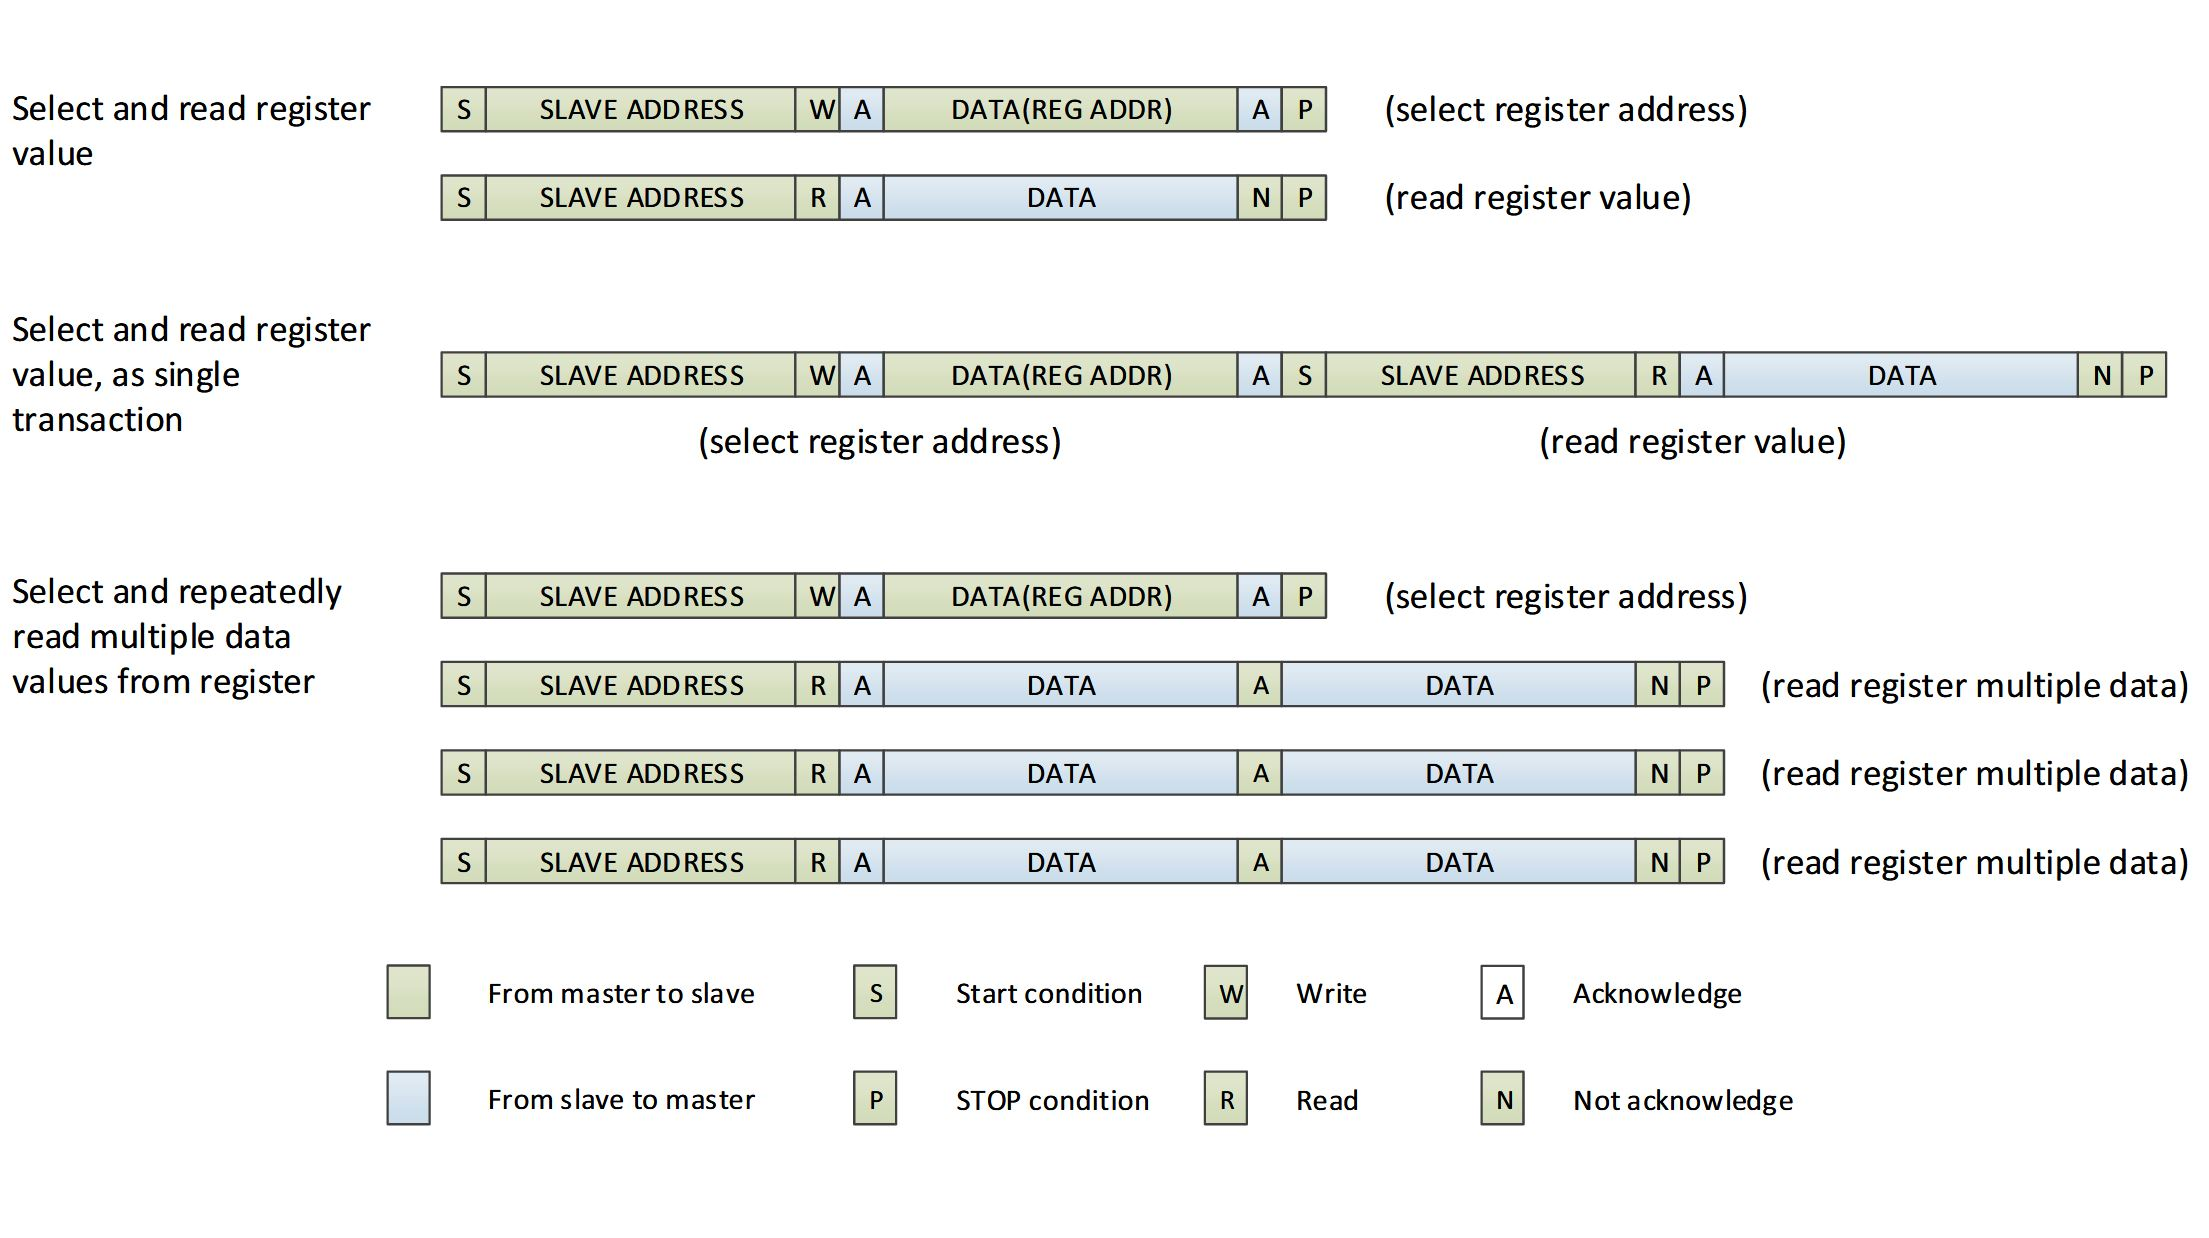
\includegraphics[scale=0.30]{images/i2c_ccs811}
	\caption{Funktionsweise der I2C-Packet Übertragung\cite{datasheetcss811}}
	\label{img:I2C_ccs811}
\end{figure}


\subsection{Achim Glaesmann}
Über die Vorlesungsfreie Zeit wurde entsprechend der Aufgabenverteilung das Auslesen des SCD41 realisiert, so wie eine Firmware entwickelt, welche in der Lage ist sowohl den SHT21 wie auch den SCD41 parallel auszulesen. Das auslesen des SCD41 bereitete zunächst enorme Schwierigkeiten. Verschiedene in der Firmware des Atmel Mikroprozessors eingebaute Funktionen verursachten schwer nachzuvollziehende Bugs. Den Versuch die I2C Schnittstelle über den Befehl HAL_CloseI2cPacket(&i2cdescriptor) an einer Stelle im Code außerhalb der Callback Funktion des Descriptors, führte zu einem Bug bei welchem in ständiger Wiederholung der Mikroprozessor neu startete. Der Neustart trat allerdings nicht an der Stelle auf an dem die Funktion aufgerufen wurde. Das Problem konnte behoben werden, nachdem die HAL_CloseI2cPacket() Funktion nur noch in der dem Descriptor zugehörigen Callbackfunktion aufgerufen wurde. Die Identifizierung des Fehlers kostete allerdings sehr viel Zeit, da Zeitpunkt der Anweisung und Auftreten des Fehlers nicht übereinstimmten.
Es war nötig eine Delay Funktion einzuführen, da die vom Hersteller gegebene Delayfunktion den Programmablauf nicht unterbrach. Da eine längere Programmunterbrechung allerdings ohnehin die vom Taskhandler regelmäßig aufzurufenden Zigbee Funktionen des Bitcloud Stack behindern würde, wurde eine Funktion auf Basis eines Timers und einer Zustandsänderung eingeführt. Die Variable appstate wurde von einem Enum zu einem Integer umdefiniert um eine einfachere Implementierung in der Delayfunktion zu ermöglichen. 

\begin{lstlisting}[language=C,frame=single, caption = Delay Timer, label = delay_timer] 
static void delaytimer(uint16_t time, uint8_t _next_appstate){
	delayTimer.interval = time;
	next_appstate = _next_appstate;
	HAL_StartAppTimer(&delayTimer) //startet timer delayTimer welcher nach der angegebenen Zeit in ms die Funktion delayTimerComplete(); aufruft
}

static void delayTimerComplete(){
appstate = next_appstate;
SYS_PostTask(APL_TASK_ID); 
}

\end{lstlisting} 

Es war daraufhin nötig Zustände, die eine Unterbrechung des Programmablaufs benötigten um die Rechenaufgaben der Sensoren zu ermöglichen, zu trennen. Es war möglich die Applikation in 10 Zustände zu unterteilen.

\begin{lstlisting}[language=C,frame=single, caption = APPSTATE definitions , label = appstate_define] 
#define APP_NOTHING_STATE				0
#define APP_STARTUP_STATE 				1
#define APP_RESET_SENSOR_STATE 			2
#define APP_INIT_STATE 				3
#define APP_CALL_FOR_READ_SCD_STATE 		4
#define APP_CALL_FOR_READ_TEMP_SHT_STATE 	5
#define APP_CALL_FOR_READ_RH_SHT_STATE 	6
#define APP_READ_SCD_STATE 			7
#define APP_READ_TEMP_SHT_STATE 		8
#define APP_READ_RH_SHT_STATE 			9
#define APP_AUSGABE_STATE 				10
\end{lstlisting} 

Die I2C Verbindung zu den einzelnen Sensoren konnte über den eingeführten Delay stabilisiert werden.
Die Kommunikation zum SCD41 warf jedoch weiterhin Fehler auf, die zunächst nicht nachvollzogen werden konnten. Nach testen des Sensors auf dem Arduino und dem recherchieren der Funktionen der von Sensirion bereitgestellten Arduino-Library wurde erkannt, das zum erfolgreichen Starten der periodischen Messung zunächst ein Reset des Sensors durchgeführt werden muss. Das unterbrechen der Stromversorgung zum Sensor scheint hierbei nicht zwingend auszureichen. Ein erneutes übersenden des Befehls zur Periodischen Messung führt ohne den vorherigen Reset dann nicht zu der erwünschten Messung. Weiterhin ist es nötig den Sensor vor der ersten I2C-Kommunikation für eine Zeit mit Strom zu versorgen damit dieser die zur Funktion nötigen Anweisungen ausführen kann. Das der Befehl nach Neustart des Sensors dennoch zurückgesetzt werden muss, war leider nicht eindeutig im Datenblatt vermerkt, weswegen auch das finden des Fehlers in dieser Kommunikation beachtliche Zeit in Anspruch nahm.
Zuletzt war es jedoch möglich beide Sensoren auszulesen und in einer Firmware zu verbinden. Nachdem meine Teamkollegen die 2.4Ghz Verbindung so wie den CCS881 erfolgreich implementiert haben ist es möglich die Firmware abschließend zu entwickeln, so dass die Sensoren in den jeweiligen Räumen platziert und mit der Applikation verbunden werden können. 



\subsection{Max-Rene Konieczka}
Während zurzeit noch daran gearbeitet wird die Daten der Sensoren auszulesen, wurde zunächst versucht die zuvor mit Python erstellten Mockdaten, in unsere Datenbank einzulesen. Dafür haben wir das Serialport Package von Node sowie ein Programm zur Erstellung von virtuellen Ports verwendet. Es hat sich die Frage gestellt, ob und wie die Mockdaten in der Datenbank angezeigt werden könnten. Das Abspeichern hat funktioniert, doch ist der Gedanke aufgekommen, dass wir die Daten direkt auf einem Modul, mit Atmel Studio erstellen sollten. Da nämlich zusätzliche Software benutzt wird, müsste diese von zukünftigen Benutzern ebenfalls heruntergeladen und installiert werden. Dies soll allerdings verhindert werden.
\subsection{Can Cihan Nazlier}
Das Abspeichern von Sensoren in den Räumen in Echtzeit, wurde nun in der Datenbank realisiert. Das heißt, sobald ein Sensor aus einem Raum entfernt wird und ein anderer hinzugefügt wird, dann bekommt das Backend dies mit und diese Information an die Datenbank weiter. Somit besteht nun eine Verbindung vom Raum und Sensor über deren ID's. Zudem wurde das Abspeichern und Abfangen der Mockdaten realisiert.
Die Mockdaten werden momentan mit Python erstellt, dies gab einigen zu Bedenken dass es ohne zusätzliche Software evtl. nicht klappen könnte in den Entwicklungsumgebungen
aller Entwickler, sodass der nächste Schritt ist, die Mockdaten via eines Zigbee Moduls zu senden. Im gleichen Schritt wird als Nächstes das Dashboard erstellt.

\printbibliography
%----------------------------------------------------------------------------
% Bibliography
%----------------------------------------------------------------------------	

\end{document}
